% Options for packages loaded elsewhere
% Options for packages loaded elsewhere
\PassOptionsToPackage{unicode}{hyperref}
\PassOptionsToPackage{hyphens}{url}
\PassOptionsToPackage{dvipsnames,svgnames,x11names}{xcolor}
%
\documentclass[
  letterpaper,
  DIV=11,
  numbers=noendperiod]{scrartcl}
\usepackage{xcolor}
\usepackage{amsmath,amssymb}
\setcounter{secnumdepth}{5}
\usepackage{iftex}
\ifPDFTeX
  \usepackage[T1]{fontenc}
  \usepackage[utf8]{inputenc}
  \usepackage{textcomp} % provide euro and other symbols
\else % if luatex or xetex
  \usepackage{unicode-math} % this also loads fontspec
  \defaultfontfeatures{Scale=MatchLowercase}
  \defaultfontfeatures[\rmfamily]{Ligatures=TeX,Scale=1}
\fi
\usepackage{lmodern}
\ifPDFTeX\else
  % xetex/luatex font selection
\fi
% Use upquote if available, for straight quotes in verbatim environments
\IfFileExists{upquote.sty}{\usepackage{upquote}}{}
\IfFileExists{microtype.sty}{% use microtype if available
  \usepackage[]{microtype}
  \UseMicrotypeSet[protrusion]{basicmath} % disable protrusion for tt fonts
}{}
\makeatletter
\@ifundefined{KOMAClassName}{% if non-KOMA class
  \IfFileExists{parskip.sty}{%
    \usepackage{parskip}
  }{% else
    \setlength{\parindent}{0pt}
    \setlength{\parskip}{6pt plus 2pt minus 1pt}}
}{% if KOMA class
  \KOMAoptions{parskip=half}}
\makeatother
% Make \paragraph and \subparagraph free-standing
\makeatletter
\ifx\paragraph\undefined\else
  \let\oldparagraph\paragraph
  \renewcommand{\paragraph}{
    \@ifstar
      \xxxParagraphStar
      \xxxParagraphNoStar
  }
  \newcommand{\xxxParagraphStar}[1]{\oldparagraph*{#1}\mbox{}}
  \newcommand{\xxxParagraphNoStar}[1]{\oldparagraph{#1}\mbox{}}
\fi
\ifx\subparagraph\undefined\else
  \let\oldsubparagraph\subparagraph
  \renewcommand{\subparagraph}{
    \@ifstar
      \xxxSubParagraphStar
      \xxxSubParagraphNoStar
  }
  \newcommand{\xxxSubParagraphStar}[1]{\oldsubparagraph*{#1}\mbox{}}
  \newcommand{\xxxSubParagraphNoStar}[1]{\oldsubparagraph{#1}\mbox{}}
\fi
\makeatother


\usepackage{longtable,booktabs,array}
\usepackage{calc} % for calculating minipage widths
% Correct order of tables after \paragraph or \subparagraph
\usepackage{etoolbox}
\makeatletter
\patchcmd\longtable{\par}{\if@noskipsec\mbox{}\fi\par}{}{}
\makeatother
% Allow footnotes in longtable head/foot
\IfFileExists{footnotehyper.sty}{\usepackage{footnotehyper}}{\usepackage{footnote}}
\makesavenoteenv{longtable}
\usepackage{graphicx}
\makeatletter
\newsavebox\pandoc@box
\newcommand*\pandocbounded[1]{% scales image to fit in text height/width
  \sbox\pandoc@box{#1}%
  \Gscale@div\@tempa{\textheight}{\dimexpr\ht\pandoc@box+\dp\pandoc@box\relax}%
  \Gscale@div\@tempb{\linewidth}{\wd\pandoc@box}%
  \ifdim\@tempb\p@<\@tempa\p@\let\@tempa\@tempb\fi% select the smaller of both
  \ifdim\@tempa\p@<\p@\scalebox{\@tempa}{\usebox\pandoc@box}%
  \else\usebox{\pandoc@box}%
  \fi%
}
% Set default figure placement to htbp
\def\fps@figure{htbp}
\makeatother


% definitions for citeproc citations
\NewDocumentCommand\citeproctext{}{}
\NewDocumentCommand\citeproc{mm}{%
  \begingroup\def\citeproctext{#2}\cite{#1}\endgroup}
\makeatletter
 % allow citations to break across lines
 \let\@cite@ofmt\@firstofone
 % avoid brackets around text for \cite:
 \def\@biblabel#1{}
 \def\@cite#1#2{{#1\if@tempswa , #2\fi}}
\makeatother
\newlength{\cslhangindent}
\setlength{\cslhangindent}{1.5em}
\newlength{\csllabelwidth}
\setlength{\csllabelwidth}{3em}
\newenvironment{CSLReferences}[2] % #1 hanging-indent, #2 entry-spacing
 {\begin{list}{}{%
  \setlength{\itemindent}{0pt}
  \setlength{\leftmargin}{0pt}
  \setlength{\parsep}{0pt}
  % turn on hanging indent if param 1 is 1
  \ifodd #1
   \setlength{\leftmargin}{\cslhangindent}
   \setlength{\itemindent}{-1\cslhangindent}
  \fi
  % set entry spacing
  \setlength{\itemsep}{#2\baselineskip}}}
 {\end{list}}
\usepackage{calc}
\newcommand{\CSLBlock}[1]{\hfill\break\parbox[t]{\linewidth}{\strut\ignorespaces#1\strut}}
\newcommand{\CSLLeftMargin}[1]{\parbox[t]{\csllabelwidth}{\strut#1\strut}}
\newcommand{\CSLRightInline}[1]{\parbox[t]{\linewidth - \csllabelwidth}{\strut#1\strut}}
\newcommand{\CSLIndent}[1]{\hspace{\cslhangindent}#1}



\setlength{\emergencystretch}{3em} % prevent overfull lines

\providecommand{\tightlist}{%
  \setlength{\itemsep}{0pt}\setlength{\parskip}{0pt}}



 


\KOMAoption{captions}{tableheading}
\makeatletter
\@ifpackageloaded{caption}{}{\usepackage{caption}}
\AtBeginDocument{%
\ifdefined\contentsname
  \renewcommand*\contentsname{Table of contents}
\else
  \newcommand\contentsname{Table of contents}
\fi
\ifdefined\listfigurename
  \renewcommand*\listfigurename{List of Figures}
\else
  \newcommand\listfigurename{List of Figures}
\fi
\ifdefined\listtablename
  \renewcommand*\listtablename{List of Tables}
\else
  \newcommand\listtablename{List of Tables}
\fi
\ifdefined\figurename
  \renewcommand*\figurename{Figure}
\else
  \newcommand\figurename{Figure}
\fi
\ifdefined\tablename
  \renewcommand*\tablename{Table}
\else
  \newcommand\tablename{Table}
\fi
}
\@ifpackageloaded{float}{}{\usepackage{float}}
\floatstyle{ruled}
\@ifundefined{c@chapter}{\newfloat{codelisting}{h}{lop}}{\newfloat{codelisting}{h}{lop}[chapter]}
\floatname{codelisting}{Listing}
\newcommand*\listoflistings{\listof{codelisting}{List of Listings}}
\makeatother
\makeatletter
\makeatother
\makeatletter
\@ifpackageloaded{caption}{}{\usepackage{caption}}
\@ifpackageloaded{subcaption}{}{\usepackage{subcaption}}
\makeatother
\usepackage{bookmark}
\IfFileExists{xurl.sty}{\usepackage{xurl}}{} % add URL line breaks if available
\urlstyle{same}
\hypersetup{
  pdftitle={Supplementary Material - Comparing Microbial Diversity and Co-Occurrence Networks Across Five Major Body Sites (HMP 16S)},
  pdfauthor={Kexin Cui},
  colorlinks=true,
  linkcolor={blue},
  filecolor={Maroon},
  citecolor={Blue},
  urlcolor={Blue},
  pdfcreator={LaTeX via pandoc}}


\title{Supplementary Material - Comparing Microbial Diversity and
Co-Occurrence Networks Across Five Major Body Sites (HMP 16S)}
\author{Kexin Cui}
\date{2026-05-06}
\begin{document}
\maketitle


\section{Overview}\label{overview}

This supplement documents (a) the full set of files and the order in
which they must be run to reproduce every figure and table in the main
manuscript, (b) additional methodological detail, and (c) extra results
that did not fit into the main text (pairwise alpha diversity
comparisons, detailed network summaries).

\section{Code and file information}\label{code-and-file-information}

The project has three code stages. Run them in the following order:

\begin{enumerate}
\def\labelenumi{\arabic{enumi}.}
\tightlist
\item
  \texttt{code/processing-code/processingfile-v1.qmd} --- downloads the
  HMP V3--V5 data with \texttt{HMP16SData::V35()}, removes zero-count
  and rare taxa, and writes \texttt{data/processed-data/ps\_filt.rds}
  and \texttt{data/processed-data/ps\_rel.rds}.
\item
  \texttt{code/eda-code/eda.qmd} --- produces the exploratory figures
  (\texttt{seq\_depth.png}, \texttt{top\_phyla.png},
  \texttt{alpha\_diversity\_5sites.png}, \texttt{shannon\_boxplot.png},
  \texttt{pcoa\_preview.png}) and the summary table
  \texttt{results/tables/exploratory\_summary\_by\_subsite.rds}.
\item
  \texttt{code/analysis-code/statistical-analysis.R} --- runs the formal
  hypothesis tests (Kruskal-Wallis, pairwise Wilcoxon, PERMANOVA,
  BETADISPER), builds per-site co-occurrence networks, and trains the
  supervised body-site classifier with cross-validation, model
  comparison and bootstrap-based uncertainty. Outputs include all tables
  (\texttt{alpha\_kruskal.rds}, \texttt{alpha\_pairwise.rds},
  \texttt{permanova.rds}, \texttt{network\_stats.rds},
  \texttt{ml\_cv\_metrics.rds}, \texttt{ml\_test\_metrics.rds},
  \texttt{ml\_test\_uncertainty.rds}, \texttt{ml\_best\_params.rds},
  \texttt{ml\_confusion\_matrix.rds},
  \texttt{ml\_variable\_importance.rds}) and figures
  (\texttt{pcoa\_ordination\_5sites.png},
  \texttt{hierarchical\_clustering\_5sites.png},
  \texttt{network\_statistics\_comparison.png},
  \texttt{ml\_cv\_comparison.png}, \texttt{ml\_confusion\_matrix.png},
  \texttt{ml\_roc\_curves.png}, \texttt{ml\_variable\_importance.png}).
\end{enumerate}

The manuscript Quarto file \texttt{products/manuscript/Manuscript.qmd}
and this supplement pull these results in via \texttt{readRDS()} and
\texttt{knitr::include\_graphics()}.

\newpage{}

\section{Additional method details}\label{additional-method-details}

\subsection{Stratified subsampling}\label{stratified-subsampling}

To make the comparison across the five major body sites balanced, we
sample up to 200 samples per site using base R's \texttt{sample()} with
\texttt{set.seed(123)}. Sites with fewer than 200 samples are included
in full. This procedure gives the same set of samples on every run.

\subsection{Filtering and rarefaction}\label{filtering-and-rarefaction}

Taxa are retained only if they are present in at least 10 samples and
have a total count of ≥ 50 reads. Samples are rarefied to the 5th
percentile of the distribution of sample sums, using
\texttt{phyloseq::rarefy\_even\_depth()} with \texttt{rngseed\ =\ 123}.
This threshold keeps 95\% of samples while substantially reducing
variation in sequencing depth.

\subsection{Distance choice}\label{distance-choice}

We use Bray-Curtis as the primary distance because it is abundance-aware
and is the default distance in most HMP-era papers. Jaccard (presence/
absence) is used as a robustness check. BETADISPER tests whether the
PERMANOVA effect is confounded with unequal dispersion among groups;
both tests are reported.

\subsection{Network construction}\label{network-construction}

Correlation networks are built per body site from the
prevalence-filtered OTU table (≥ 10\% prevalence) using Spearman
correlations via \texttt{Hmisc::rcorr}. Edges are retained when
\textbar r\textbar{} ≥ 0.5 and p \textless{} 0.01 (no multiple-testing
correction is applied inside the network --- this is a pragmatic
threshold, not a formal significance test). Louvain community detection
(\texttt{igraph::cluster\_louvain}) is used to compute modularity and
communities.

\subsection{Supervised classification
(H4)}\label{supervised-classification-h4}

The H4 pipeline showcases several data-science topics from the course in
one place: model fitting and tuning, cross-validation, model comparison,
regularization, ensemble methods, calibration via ROC curves, variable
importance, and uncertainty quantification.

\begin{itemize}
\tightlist
\item
  \emph{Features.} The 300 most-abundant taxa, log(1 + x)-transformed
  and z-scored. Constant-zero predictors are removed with
  \texttt{step\_zv}.
\item
  \emph{Resampling.} A 75/25 stratified train/test split, with 5-fold
  cross-validation on the training set, also stratified by body site.
\item
  \emph{Candidate models.} Five workflows:

  \begin{enumerate}
  \def\labelenumi{\arabic{enumi}.}
  \tightlist
  \item
    \texttt{parsnip::null\_model} --- baseline that always predicts the
    modal class.
  \item
    \texttt{multinom\_reg} (glmnet) --- elastic-net regularized
    multinomial logistic regression; \texttt{penalty} swept on a
    log-grid from 1e-4 to 1 and \texttt{mixture} swept from 0 (ridge) to
    1 (lasso).
  \item
    \texttt{decision\_tree} (rpart) --- single CART;
    \texttt{cost\_complexity} from 1e-4 to 1e-1, \texttt{tree\_depth}
    from 3 to 15, and \texttt{min\_n} from 2 to 20.
  \item
    \texttt{rand\_forest} (ranger, 500 trees,
    \texttt{importance\ =\ "permutation"}) --- \texttt{mtry} swept on
    \{5, 35, 70, 100\} and \texttt{min\_n} on \{2, 8, 14, 20\}.
  \item
    \texttt{boost\_tree} (xgboost) --- \texttt{trees} \{100, 800\},
    \texttt{tree\_depth} \{3, 9\}, \texttt{learn\_rate} swept on a
    log-grid from 1e-2 to \textasciitilde3e-1, and \texttt{min\_n} \{2,
    20\}. Skipped automatically when \texttt{xgboost} is not installed.
  \end{enumerate}
\item
  \emph{Selection.} For each model we pick the hyperparameter setting
  that maximizes mean macro-AUC across the 5 folds, then refit on the
  full training set and evaluate on the held-out test set.
\item
  \emph{Uncertainty.} Test-set accuracy and macro-AUC are bootstrapped
  on the predictions: 1000 resamples (with replacement) of the per-row
  prediction tibble, and the 2.5\%/97.5\% quantiles serve as the 95\%
  confidence interval.
\item
  \emph{Variable importance.} For the winning model, we extract the
  top-20 features by \texttt{vip::vi}, which uses the engine-native
  importance (permutation importance for ranger, gain for xgboost, and
  absolute coefficient size for glmnet).
\end{itemize}

\newpage{}

\section{Additional results}\label{additional-results}

\subsection{Pairwise alpha diversity
comparisons}\label{pairwise-alpha-diversity-comparisons}

Table Table~\ref{tbl-alpha-pairwise} lists the
Benjamini-Hochberg-adjusted pairwise Wilcoxon p-values for every pair of
body sites, for each of the four alpha-diversity indices. These follow
up the overall Kruskal-Wallis tests reported in the main text.

\begin{longtable}[]{@{}lllr@{}}

\caption{\label{tbl-alpha-pairwise}Pairwise Wilcoxon (BH-adjusted)
p-values for alpha diversity differences across body sites.}

\tabularnewline

\toprule\noalign{}
metric & site\_1 & site\_2 & p\_adj \\
\midrule\noalign{}
\endhead
\bottomrule\noalign{}
\endlastfoot
Observed & Gut & Airways & 0 \\
Observed & Oral & Airways & 0 \\
Observed & Skin & Airways & 0 \\
Observed & Urogenital & Airways & 0 \\
Observed & Oral & Gut & 0 \\
Observed & Skin & Gut & 0 \\
Observed & Urogenital & Gut & 0 \\
Observed & Skin & Oral & 0 \\
Observed & Urogenital & Oral & 0 \\
Observed & Urogenital & Skin & 0 \\
Shannon & Gut & Airways & 0 \\
Shannon & Oral & Airways & 0 \\
Shannon & Skin & Airways & 0 \\
Shannon & Urogenital & Airways & 0 \\
Shannon & Oral & Gut & 0 \\
Shannon & Skin & Gut & 0 \\
Shannon & Urogenital & Gut & 0 \\
Shannon & Skin & Oral & 0 \\
Shannon & Urogenital & Oral & 0 \\
Shannon & Urogenital & Skin & 0 \\
Simpson & Gut & Airways & 0 \\
Simpson & Oral & Airways & 0 \\
Simpson & Skin & Airways & 0 \\
Simpson & Urogenital & Airways & 0 \\
Simpson & Oral & Gut & 0 \\
Simpson & Skin & Gut & 0 \\
Simpson & Urogenital & Gut & 0 \\
Simpson & Skin & Oral & 0 \\
Simpson & Urogenital & Oral & 0 \\
Simpson & Urogenital & Skin & 0 \\
Chao1 & Gut & Airways & 0 \\
Chao1 & Oral & Airways & 0 \\
Chao1 & Skin & Airways & 0 \\
Chao1 & Urogenital & Airways & 0 \\
Chao1 & Oral & Gut & 0 \\
Chao1 & Skin & Gut & 0 \\
Chao1 & Urogenital & Gut & 0 \\
Chao1 & Skin & Oral & 0 \\
Chao1 & Urogenital & Oral & 0 \\
Chao1 & Urogenital & Skin & 0 \\

\end{longtable}

\subsection{Full network statistics}\label{full-network-statistics}

Table Table~\ref{tbl-network-full} provides the full per-site network
statistics (reproduced here from the main text for convenience, together
with the number of positive vs.~negative edges that are not shown in the
main figure).

\begin{longtable}[]{@{}
  >{\raggedright\arraybackslash}p{(\linewidth - 14\tabcolsep) * \real{0.1467}}
  >{\raggedleft\arraybackslash}p{(\linewidth - 14\tabcolsep) * \real{0.0800}}
  >{\raggedleft\arraybackslash}p{(\linewidth - 14\tabcolsep) * \real{0.0800}}
  >{\raggedleft\arraybackslash}p{(\linewidth - 14\tabcolsep) * \real{0.1067}}
  >{\raggedleft\arraybackslash}p{(\linewidth - 14\tabcolsep) * \real{0.1333}}
  >{\raggedleft\arraybackslash}p{(\linewidth - 14\tabcolsep) * \real{0.1467}}
  >{\raggedleft\arraybackslash}p{(\linewidth - 14\tabcolsep) * \real{0.1467}}
  >{\raggedleft\arraybackslash}p{(\linewidth - 14\tabcolsep) * \real{0.1600}}@{}}

\caption{\label{tbl-network-full}Per-site co-occurrence network
summary.}

\tabularnewline

\toprule\noalign{}
\begin{minipage}[b]{\linewidth}\raggedright
BodySite
\end{minipage} & \begin{minipage}[b]{\linewidth}\raggedleft
Nodes
\end{minipage} & \begin{minipage}[b]{\linewidth}\raggedleft
Edges
\end{minipage} & \begin{minipage}[b]{\linewidth}\raggedleft
Density
\end{minipage} & \begin{minipage}[b]{\linewidth}\raggedleft
AvgDegree
\end{minipage} & \begin{minipage}[b]{\linewidth}\raggedleft
Clustering
\end{minipage} & \begin{minipage}[b]{\linewidth}\raggedleft
Modularity
\end{minipage} & \begin{minipage}[b]{\linewidth}\raggedleft
Communities
\end{minipage} \\
\midrule\noalign{}
\endhead
\bottomrule\noalign{}
\endlastfoot
Airways & 133 & 246 & 0.028 & 3.699 & 0.693 & 0.859 & 27 \\
Gut & 152 & 206 & 0.018 & 2.711 & 0.585 & 0.897 & 35 \\
Oral & 163 & 215 & 0.016 & 2.638 & 0.440 & 0.836 & 33 \\
Skin & 102 & 187 & 0.036 & 3.667 & 0.521 & 0.807 & 15 \\
Urogenital & 165 & 1411 & 0.104 & 17.103 & 0.689 & 0.672 & 6 \\

\end{longtable}

\subsection{Individual network
visualizations}\label{individual-network-visualizations}

The networks themselves are saved as an \texttt{igraph} list in
\texttt{results/output/networks.rds}. Each network can be loaded
individually and visualized with \texttt{ggraph}; below is a placeholder
for a figure panel showing one representative network per body site.

\begin{figure}

\centering{

\includegraphics[width=12in,height=\textheight,keepaspectratio]{../../../results/figures/network_statistics_comparison.png}

}

\caption{\label{fig-network-oral}Representative co-occurrence network
visualization (replace with a saved network PNG).}

\end{figure}%

\subsection{Cross-validation comparison and tuned
hyperparameters}\label{cross-validation-comparison-and-tuned-hyperparameters}

Table Table~\ref{tbl-ml-cv-supp} gives the full cross-validation summary
across the five candidate models, and Table
Table~\ref{tbl-ml-best-params} lists the hyperparameters selected by
\texttt{select\_best(metric\ =\ "roc\_auc")} for each non-null model.

\begin{longtable}[]{@{}lrrrl@{}}

\caption{\label{tbl-ml-cv-supp}Cross-validation accuracy and macro-AUC
for every candidate model (mean +/- SD across folds).}

\tabularnewline

\toprule\noalign{}
.metric & mean & sd & n & model \\
\midrule\noalign{}
\endhead
\bottomrule\noalign{}
\endlastfoot
accuracy & 0.208 & 0.002 & 5 & null \\
roc\_auc & 0.500 & 0.000 & 5 & null \\
accuracy & 0.966 & 0.009 & 5 & multinom\_glmnet \\
roc\_auc & 0.996 & 0.005 & 5 & multinom\_glmnet \\
accuracy & 0.876 & 0.014 & 5 & decision\_tree \\
roc\_auc & 0.961 & 0.011 & 5 & decision\_tree \\
accuracy & 0.962 & 0.014 & 5 & random\_forest \\
roc\_auc & 0.996 & 0.002 & 5 & random\_forest \\

\end{longtable}

\begin{longtable}[]{@{}lll@{}}

\caption{\label{tbl-ml-best-params}Tuned hyperparameter values selected
on cross-validation macro-AUC.}

\tabularnewline

\toprule\noalign{}
model & param & value \\
\midrule\noalign{}
\endhead
\bottomrule\noalign{}
\endlastfoot
multinom\_glmnet & penalty & 0.268269579527972 \\
multinom\_glmnet & mixture & 0 \\
decision\_tree & cost\_complexity & 1e-04 \\
decision\_tree & tree\_depth & 15 \\
decision\_tree & min\_n & 20 \\
random\_forest & mtry & 5 \\
random\_forest & min\_n & 2 \\

\end{longtable}

\subsection{Test-set ROC curves and bootstrap
uncertainty}\label{test-set-roc-curves-and-bootstrap-uncertainty}

Figure Figure~\ref{fig-ml-roc-supp} shows the per-class ROC curves for
the winning model, and Table Table~\ref{tbl-ml-uncert-supp} reports
bootstrap 95\% confidence intervals on test accuracy and macro-AUC (B =
1000 resamples). The CIs are narrow on this dataset, which reflects the
large held-out test sample and the strong signal in the features.

\begin{figure}

\centering{

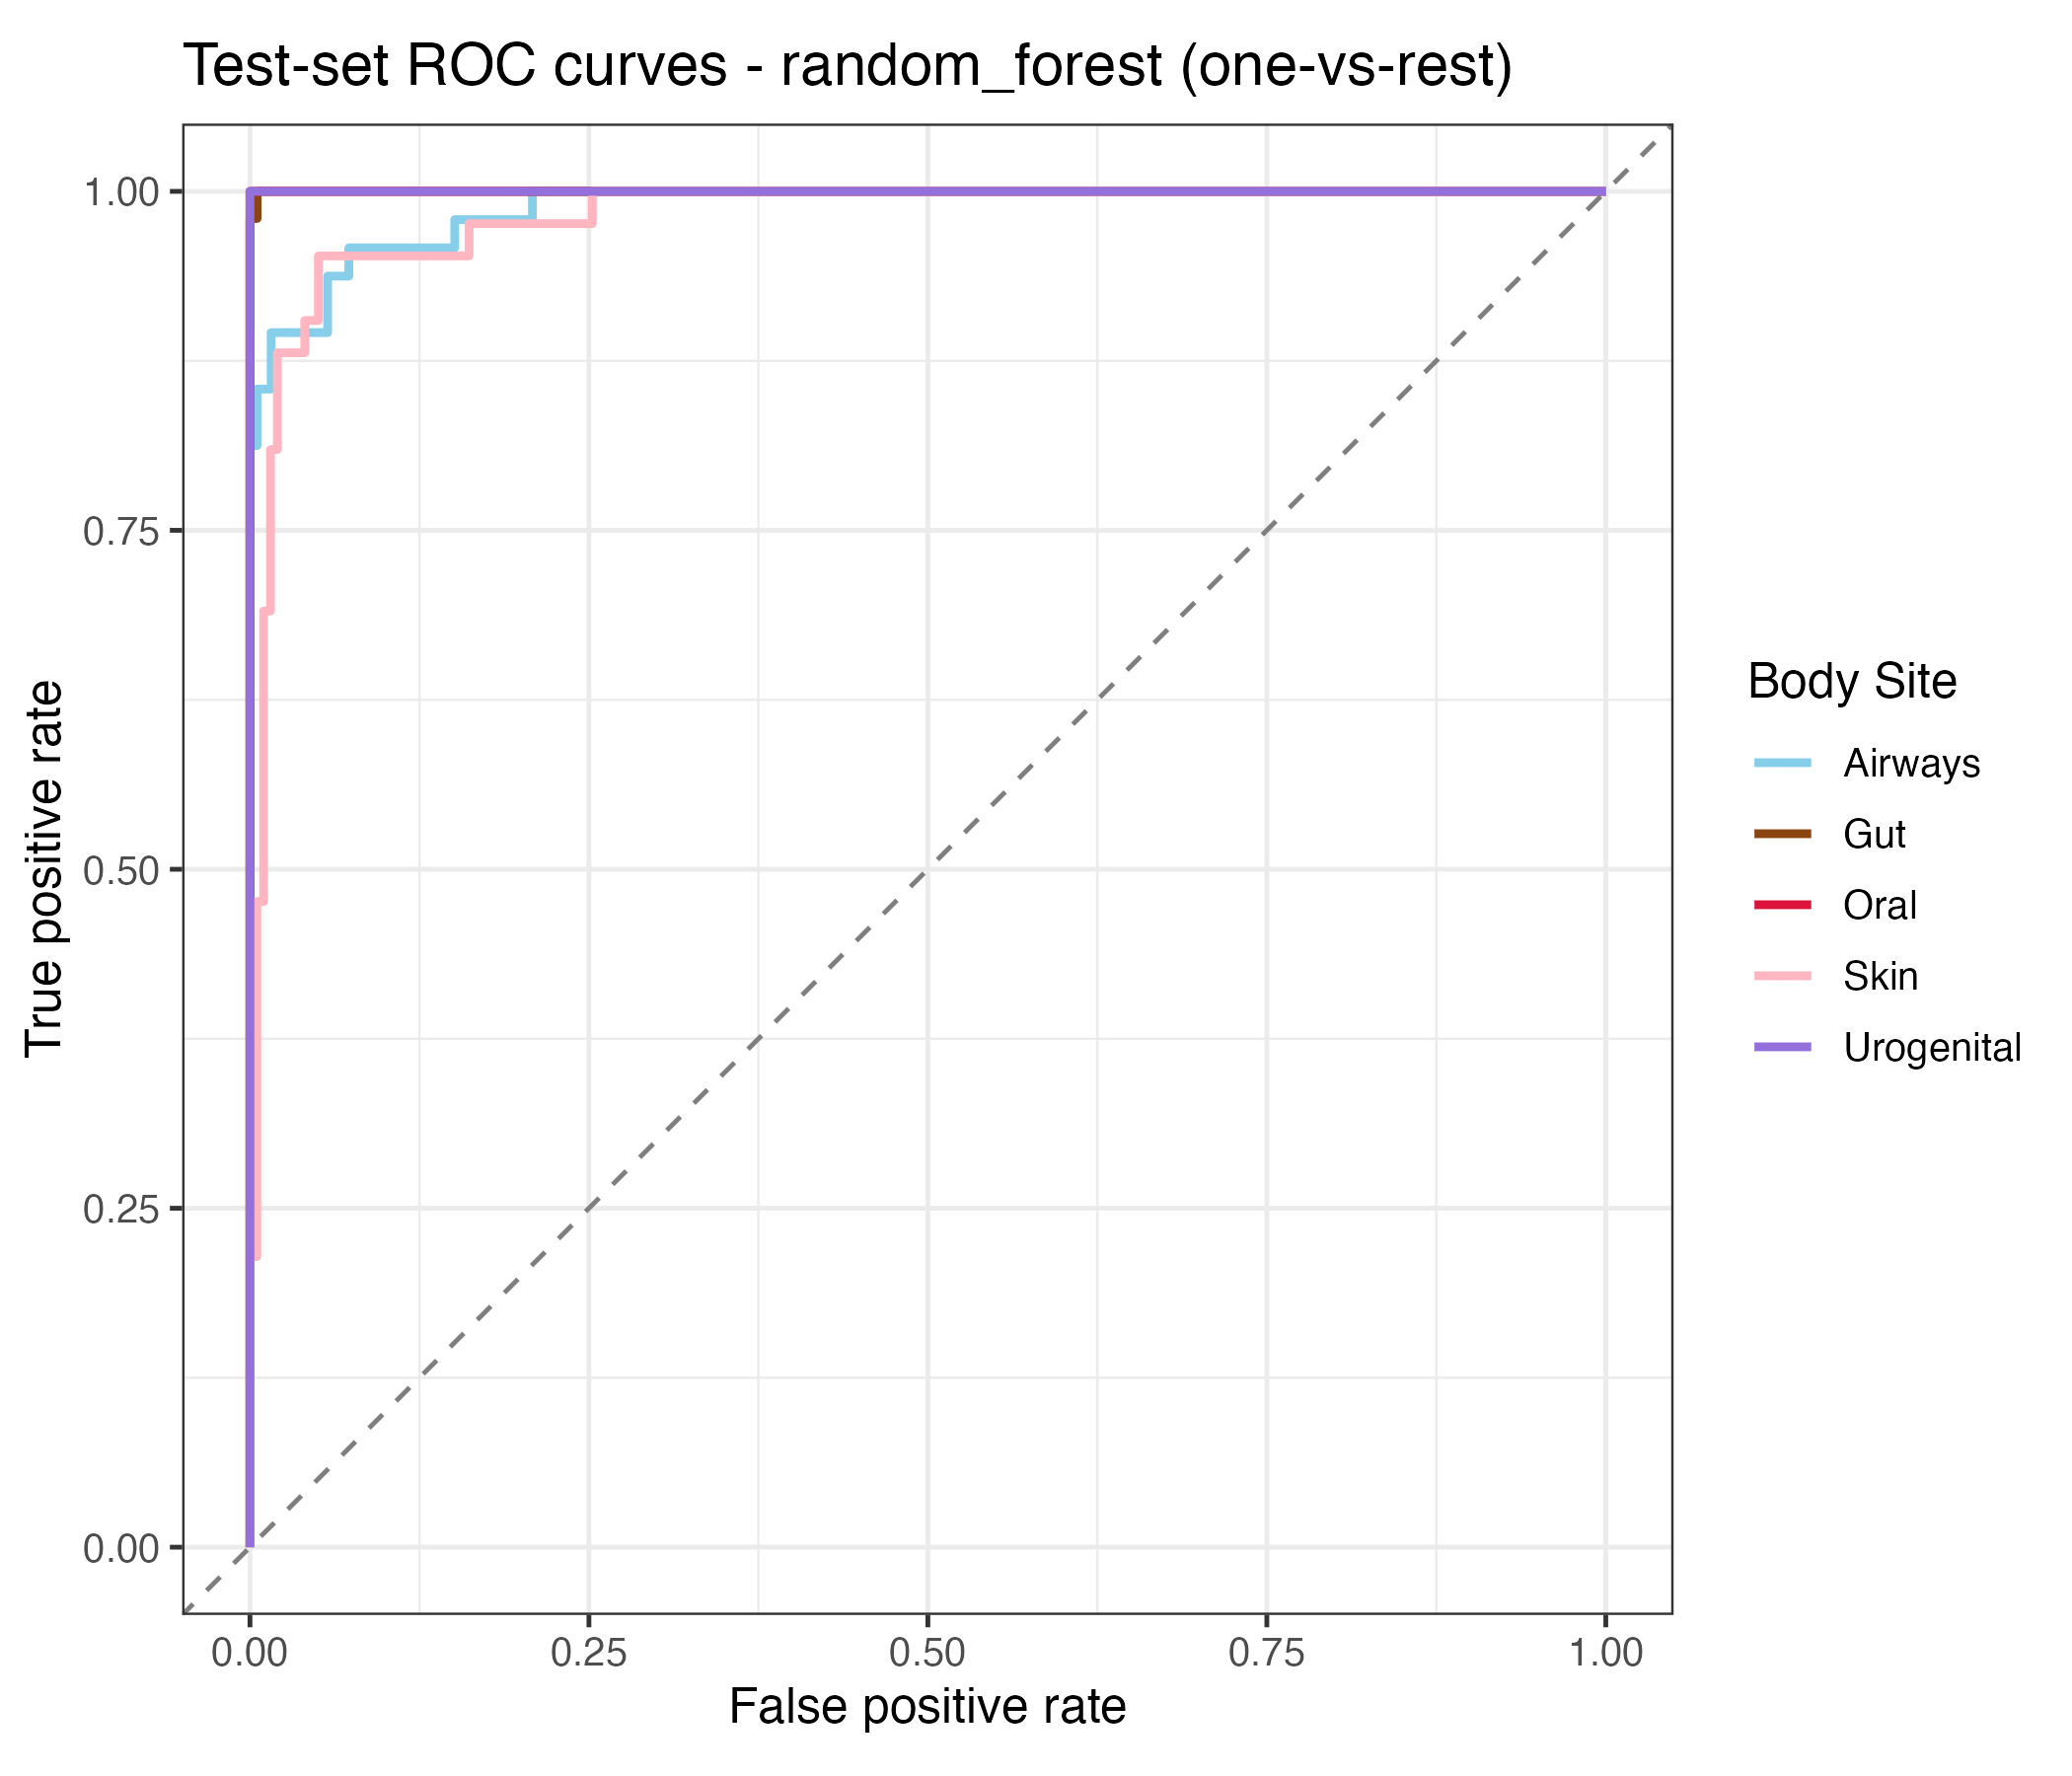
\includegraphics[width=7in,height=\textheight,keepaspectratio]{../../../results/figures/ml_roc_curves.png}

}

\caption{\label{fig-ml-roc-supp}Test-set one-vs-rest ROC curves for the
winning classifier.}

\end{figure}%

\begin{longtable}[]{@{}lrrrlr@{}}

\caption{\label{tbl-ml-uncert-supp}Bootstrap 95\% CIs on test-set
accuracy and macro-AUC (winning model).}

\tabularnewline

\toprule\noalign{}
metric & point & lower & upper & model & n\_boot \\
\midrule\noalign{}
\endhead
\bottomrule\noalign{}
\endlastfoot
accuracy & 0.958 & 0.929 & 0.979 & random\_forest & 1000 \\
roc\_auc & 0.993 & 0.988 & 0.997 & random\_forest & 1000 \\

\end{longtable}

\subsection{Variable importance}\label{variable-importance}

\begin{figure}

\centering{

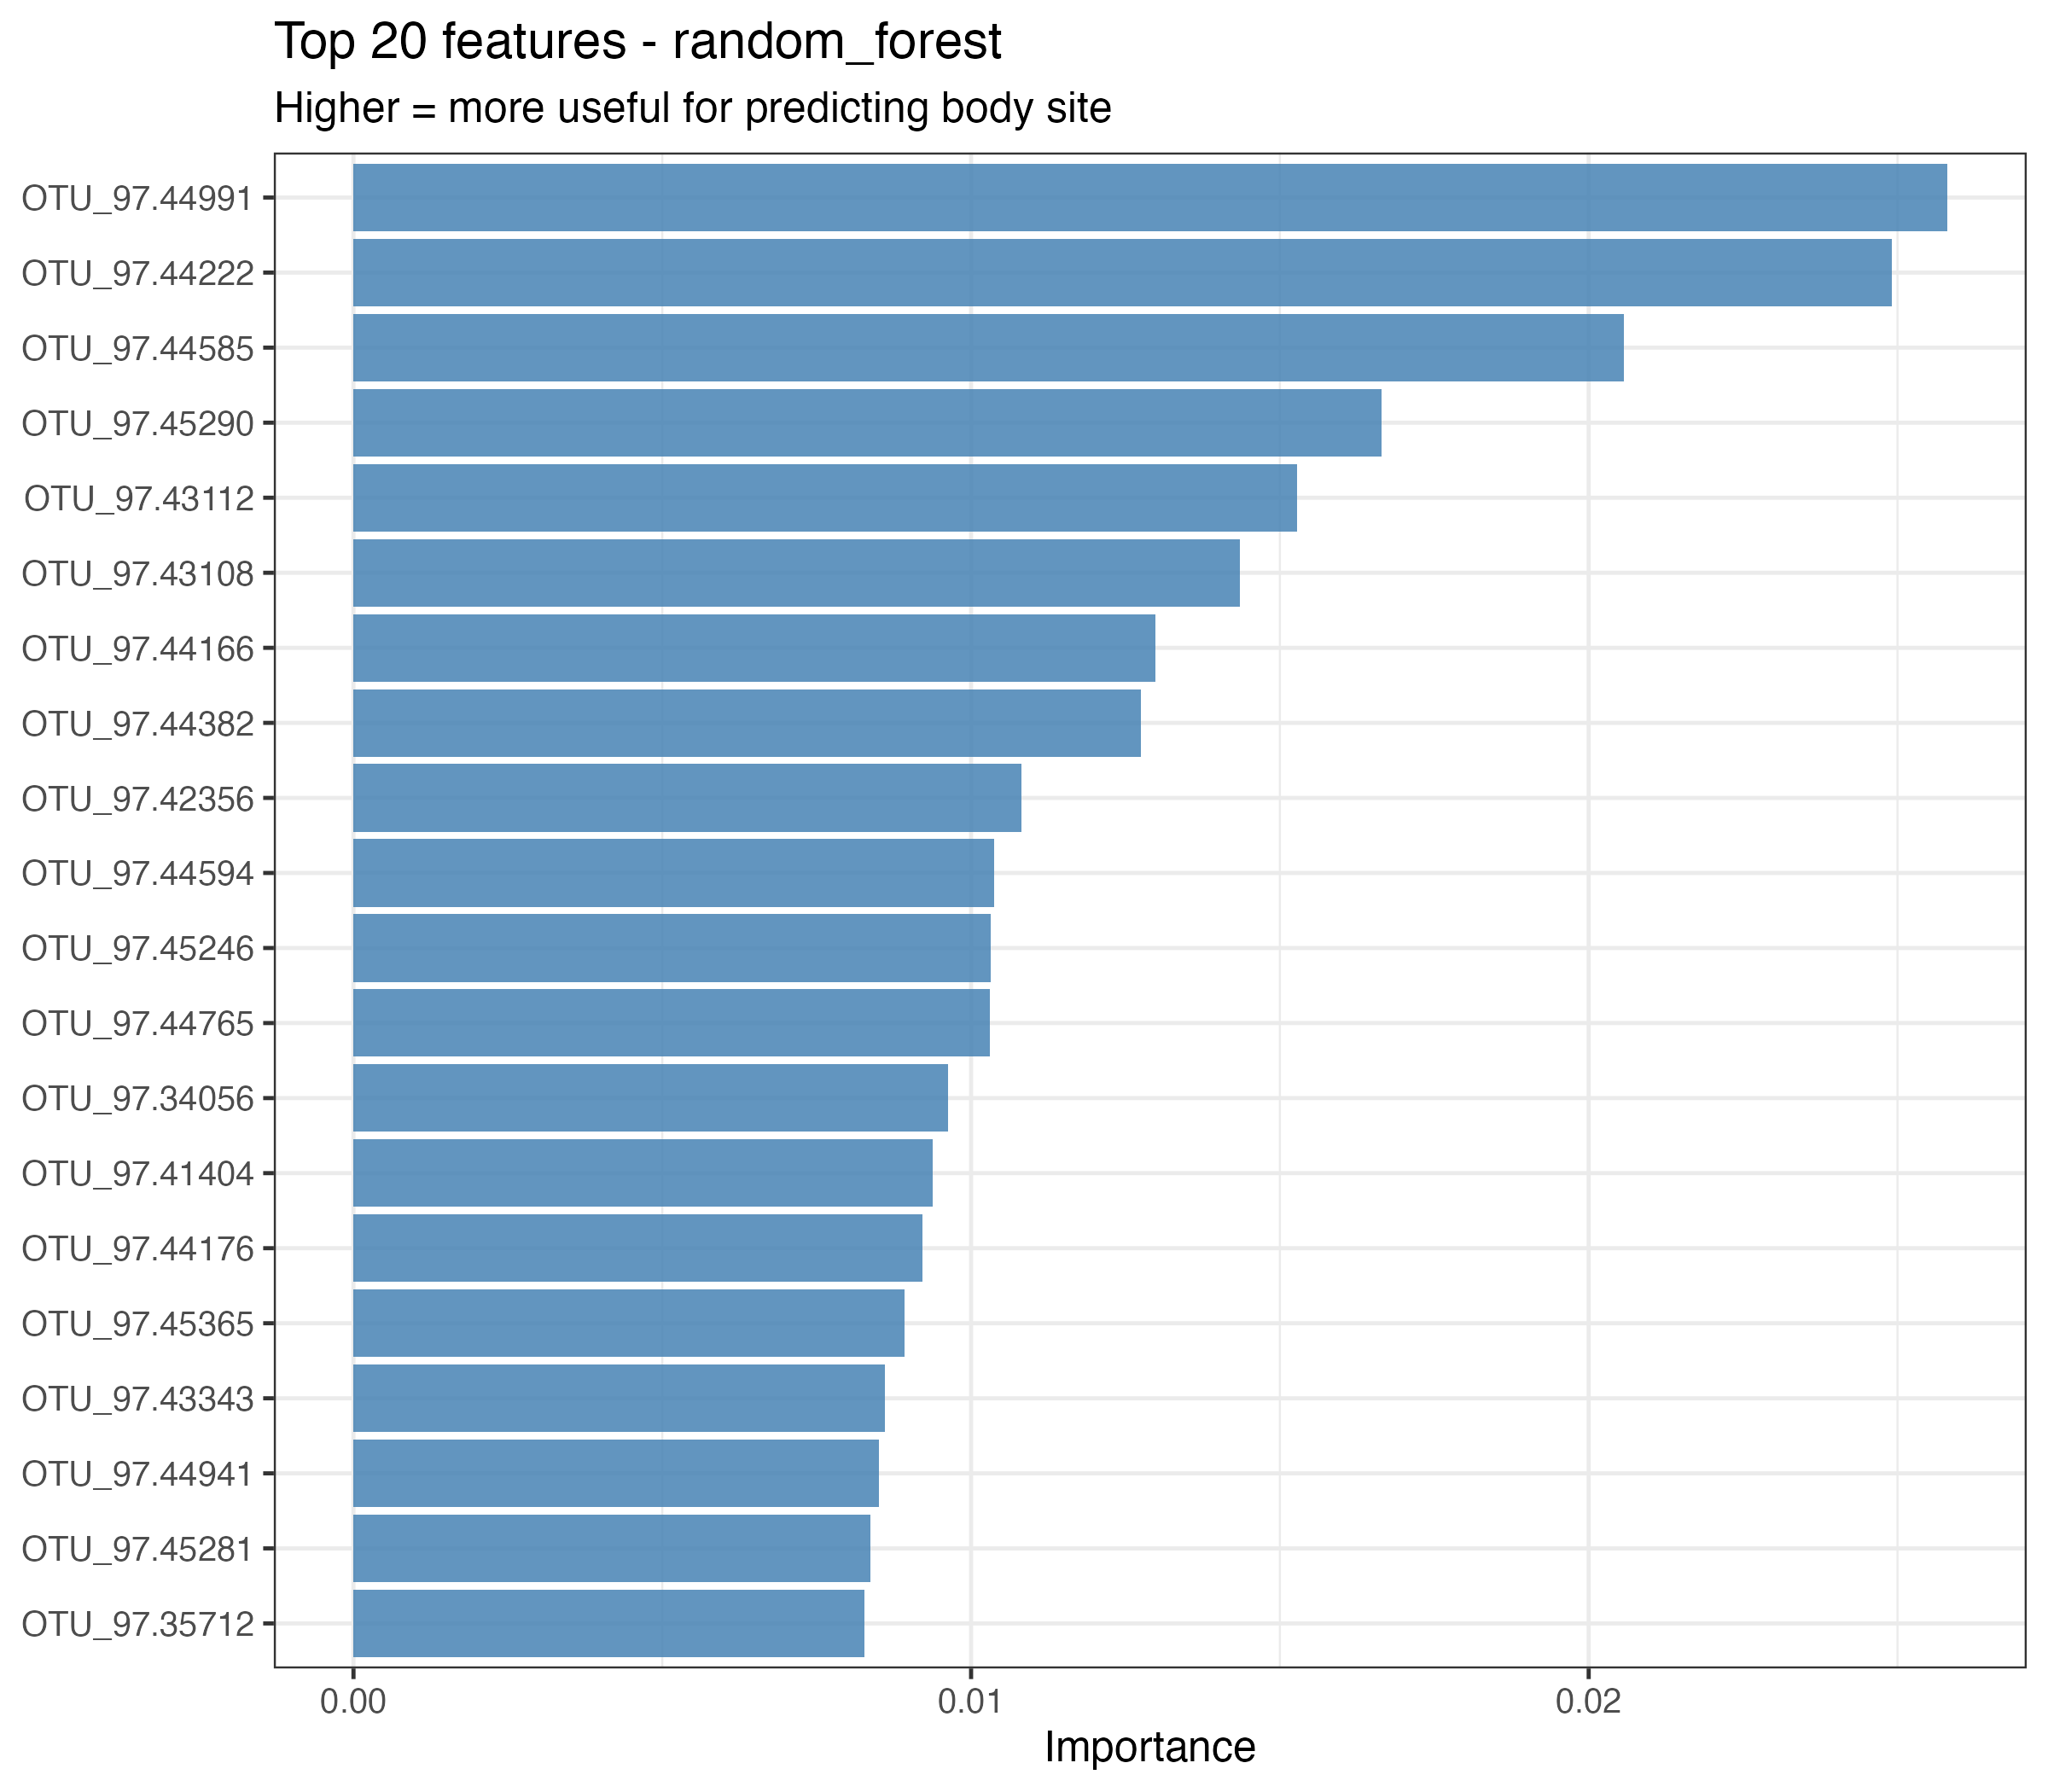
\includegraphics[width=8in,height=\textheight,keepaspectratio]{../../../results/figures/ml_variable_importance.png}

}

\caption{\label{fig-ml-vip-supp}Top 20 features (taxa) for the winning
classifier, ranked by importance.}

\end{figure}%

\newpage{}

\section{Discussion}\label{discussion}

Results in this supplement support the three main-text conclusions: (1)
the overall Kruskal-Wallis tests are not driven by a single outlier site
--- most pairwise contrasts are significant after BH correction; (2)
PERMANOVA effects are robust to switching between Bray-Curtis and
Jaccard distances; and (3) network differences across sites are not
artifacts of sample size alone, because the ranking of sites by
modularity and communities is consistent with the ecological structure
reported in the literature (McKay et al. 2020a, 2020b).

\newpage{}

\section*{References}\label{references}
\addcontentsline{toc}{section}{References}

\phantomsection\label{refs}
\begin{CSLReferences}{1}{1}
\bibitem[\citeproctext]{ref-mckay2020}
McKay B, Ebell M, Billings WZ, Dale AP, Shen Y, Handel A.
\href{https://doi.org/10.1093/ofid/ofaa494}{Associations {Between
Relative Viral Load} at {Diagnosis} and {Influenza A Symptoms} and
{Recovery}.} Open forum infectious diseases. 2020 Nov a;7(11):ofaa494.

\bibitem[\citeproctext]{ref-mckay2020a}
McKay B, Ebell M, Dale AP, Shen Y, Handel A.
\href{https://doi.org/10.1098/rspb.2020.0496}{Virulence-mediated
infectiousness and activity trade-offs and their impact on transmission
potential of influenza patients.} Proceedings Biological sciences. 2020
May b;287(1927):20200496.

\end{CSLReferences}




\end{document}
